\tikzstyle{arrow} = [thick,->,>=stealth]
    \tikzstyle{cycle} = [
        rectangle,
        minimum width=3cm,
        minimum height=1cm,
        text width=3cm,
        text centered,
        draw=black,
        fill=orange!30
    ]
    \tikzstyle{geste} = [
        rectangle,
        minimum width=3cm,
        minimum height=1cm,
        text width=3cm,
        text centered,
        draw=black,
        fill=green!30
    ]
    \tikzstyle{chanson} = [
        rectangle,
        minimum width=3cm,
        minimum height=1cm,
        text width=3cm,
        text centered,
        draw=black,
        fill=blue!30
    ]
    \tikzstyle{witness} = [
        rectangle,
        minimum width=3cm,
        minimum height=1cm,
        text width=3cm,
        text centered,
        draw=black,
        fill=cyan!30
    ]
    \tikzstyle{doc} = [
        rectangle,
        minimum width=3cm,
        minimum height=1cm,
        text width=3cm,
        text centered,
        draw=black,
        fill=red!30
    ]

\begin{frame}{Inter-entity relationships}

    \centering
    
    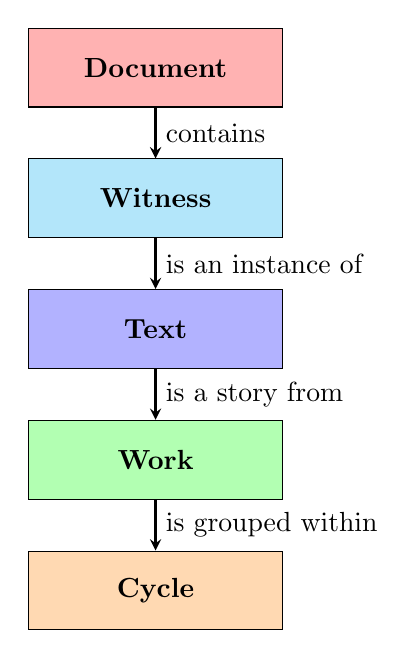
\begin{tikzpicture}[node distance=1.66cm]
        \node[doc] (document) {\textbf{Document}};
        \node[witness, below of=document] (witness) {\textbf{Witness}};
        \node[chanson, below of=witness] (chanson) {\textbf{Text}};
        \node[geste, below of=chanson] (geste) {\textbf{Work}};
        \node[cycle, below of=geste] (cycle) {\textbf{Cycle}};

        \draw[arrow] (geste) -- (cycle) node[midway, right] {is grouped within};
        \draw[arrow] (chanson) -- (geste) node[midway, right] {is a story from};
        \draw[arrow] (witness) -- (chanson) node[midway, right]{is an instance of};
        \draw[arrow] (document) -- (witness) node[midway, right]{contains};
    \end{tikzpicture}

\end{frame}

\begin{frame}{Cycle-to-cycle relationships}

    A cycle can be related to another cycle.

    \begin{center}
    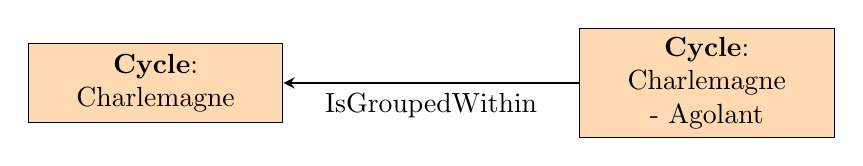
\begin{tikzpicture}[node distance=7cm]
        \node [cycle] (cycle1) {\textbf{Cycle}:\\Charlemagne};
        \node [cycle, right of=cycle1] (cycle2) {\textbf{Cycle}:\\Charlemagne - Agolant};
        \draw [arrow] (cycle2) -- (cycle1) node[midway, below]{IsGroupedWithin};
    \end{tikzpicture}
    \end{center}

    
\end{frame}

\begin{frame}{Text-to-text relationships}

    A text can be derivative of / related to another text in multiple ways.

    \begin{center}
    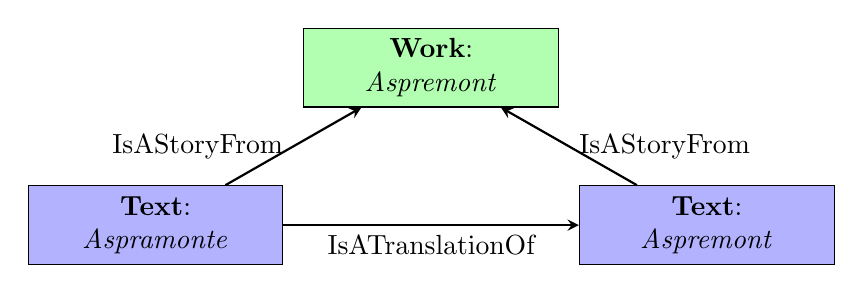
\begin{tikzpicture}[node distance=2cm]
        \node [chanson] (text1) {\textbf{Text}:\\\textit{Aspramonte}};
        \node [chanson, right of=text1, xshift=5cm] (text2) {\textbf{Text}:\\\textit{Aspremont}};
        \draw [arrow] (text1) -- (text2) node[midway, below]{IsATranslationOf};
        \node [geste, above of=text1, xshift=3.5cm] (geste) {\textbf{Work}:\\\textit{Aspremont}};
        \draw [arrow] (text1) -- (geste) node[midway, left]{IsAStoryFrom};
        \draw [arrow] (text2) -- (geste) node[midway, right]{IsAStoryFrom};
    \end{tikzpicture}
    \end{center}

    \vspace{1em}
    Text A is \ldots Text B:

    \begin{itemize}
        \item is a \textit{version} of [inverse: is a \textit{model} for]
        \item is a \textit{translation}
        \item is a \textit{prosification} of [inverse: is a \textit{reversification} of]
        \item is an \textit{abridgement} of [inverse: is an \textit{amplification} of]
    \end{itemize}

    \vspace{1em}
    
\end{frame}